% !TEX root = proposal.tex
\section{Background and Related Work}
\label{sec:related}

In this section, I discuss related work and present my previous research
results relevant to my thesis to help reader to identify the context of this
thesis proposal.

\subsection{Related Work}

\subsubsection{Inline Monitors}
\label{ssec:inline}

Program protection and profiling using inline monitors are dynamic analysis
approaches that execute specific analysis logics along with the application
process. Instance of the technology includes data flow tracking
(DFT)~\cite{DFT}, memory integrity checking~\cite{memcheck}, control flow
integrity~\cite{cfi}, method counting, call graph profiling and so on.
Given that the technology can be implemented interleaving analysis/monitoring
logics into the program execution, we can choose different instrumentation
targets either of source code or program binaries and use different
instrumentation mediums to implement inline monitors.

Employing source code based approach, we can use representations
exposed~\cite{AST,LLVM-IR} by compiler internals as instrumentation targets or
source-to-source approaches~\cite{txl, cil} to make changes to source code.
This approach comes in reasonable amount of overhead roughly around $2\times$
or less, but it is limited in completeness not being able to support COTS
binaries (\ie 3rd party libraries).  An alternative can be binary
implementation approaches either based on process-wide virtualization using
dynamic binary instrumentation(DBI)~\cite{PIN, dynamoRIO, valgrind} or
system-wide virtualization~\cite{qemu,xen}. These address coverage issue as
these can handle unknown program binaries. However, it comes with excessive
amount of overhead which vary from $\times 5 \sim \times 100$ based on analyses
and application domains. Hardware assisted implementation~\cite{HARD, lba} can
implement inline monitors with minimal amount of overhead less than 5\% at most
supporting full coverage, but the we have not yet seen this functionality
supported by major vendors with their commodity production.

\subsubsection{Data Flow Tracking (DFT)}

DFT is one of inline monitoring approaches that accurately tracks selected data
of interest, as they flow during program execution. Among other uses, DFT has
been employed to provide insight in the behavior of applications and systems,
and to assist in the identification of configuration errors. Most prominently,
it has been used in the security field to defend against various software
exploits~\cite{}, and to enforce information flow by monitoring and restricting
the use of sensitive data~\cite{}. For the former, the network is usually
defined as the source of interesting or “tainted” data, while the use of
tainted data is disallowed in certain program locations (\eg, in instructions
manipulating the control flow of programs, such as indirect branch instructions
and function calls). For the latter, the developer or the user is responsible
for specifying the data that needs to be tracked and the restrictions on their
use. DFT is even used to assist solving performance problems~\cite{} pairing
configuration file entries with performance bottlenecks as sources and sinks. 

DFT is implemented by having shadow context that corresponds to the original
execution context. The shadow context comprise of shadow operations and shadow
memory area. Table~\ref{tab:dft_tracking} shows how instructions' DFT semantics
for general purpose instruction architecture (ISA) are defined to perform DFT
operations to keep track of changes from shadow memory area. 

\begin{table}[h]
        \centering
\begin{tabular}{|l|l|}
\hline
{\bf Instruction} & {\bf Tag propagation rule} \\ \hline \hline
    {\tt \specialcell{ALU-OP OP1 $\leftarrow$ OP2 \\ (add, sub \dots)}} & 
    {\tt t(op1) $\vert=$ t(op2)}\\ \hline
    {\tt MOV OP1  $\leftarrow$  OP2} & {\tt t(op1) = t(op2)}     \\ \hline
    {\tt LOAD OP1 $\leftarrow$ [OP2]} & {\tt t(OP1) = t([OP2])}  \\ \hline
    {\tt STORE [OP1] $\leftarrow$ OP2} & {\tt t([OP1]) = t(OP2)} \\ \hline
\end{tabular}
\caption{presents an interpretation of DFT semantics for pseudo instruction set
architecture.}
\label{tab:dft_tracking}
\end{table}

The specifics of DFT can vary significantly depending on ones goals,
performance considerations, and deployment platform. One possible
classification of existing mechanisms can be made based on the means by which
the tracking logic is augmented on regular program execution. As we discussed
from Section~\ref{ssec:inline}, DFT can be performed by inserting data tracking
logic statically during the compilation of software, or by performing source-
to-source code transformation~\cite{}. It can also be applied dynamically by
augmenting instrumentation code on existing binaries using dynamic binary
instrumentation (DBI)~\cite{}  or a modified virtual machine (VM)~\cite{}.
Finally, DFT can be also performed in hardware~\cite{}.

\subsubsection{Parallelized Analysis}
\label{ssec:parallel}

The idea of decoupling dynamic program analyses from execution, to run them in
parallel, has been studied in past in various contexts~\cite{} . 
%
Aftersight~\cite{}, ReEmu~\cite{}, and Paranoid Android~\cite{} leverage record
and replay for recording execution and replaying it, along with the analysis,
on a remote host or a different CPU (replica). They are mostly geared toward
off-line analyses and can greatly reduce the overhead imposed on the
application.  However, the speed of the analysis itself is not improved, since
execution needs to be replayed and augmented with the analysis code on the
replica.  SuperPin~\cite{} and Speck~\cite{} use speculative execution to run
application and (in-lined) analysis code in multiple threads that execute in
parallel. These systems sacrifice significant processing power to achieve speed
up.  Furthermore, handling multi-threaded applications without hardware support
remains a challenging issue for this approach. CAB~\cite{} and PiPA~\cite{} aim
at offloading the analysis code alone to another execution thread, and they are
the closed to \sreplica. However, neither of the two has been able to deliver
the expected performance gains, due to {\it (i)} naively collecting information
from the application, and {\it (ii)} the high overhead of communicating it to
the analysis thread(s). 

\subsection{Previous Research}

From my previous research, I have addressed the high overhead issue inherent to
heavy-weighted inline monitors such as DFT implementations.

\subsubsection{\libdft}

\libdft is a highly optimized DFT framework that shows comparable to or faster
performance than most previous DFT implementations. \libdft implements
instruction level monitors by instrumenting DFT instruction that perform shadow
operations against {\tt x86} binary stream at runtime using PIN~\cite{} DBI
framework.
%
\libdft's performance gain comes in two folds. 

The first optimization is by having {\it inline-friendly} DFT operations. To
interleave codes from two different contexts, underlying DBI framework should
add management instructions to save and restore states relevant to each context
for every instrumentation. The state includes the whole CPU registers and the
operation of spilling/re-filling these is typically expensive. {\it
Instrumentation inlining}~\cite{} reduces this overhead taking advantage of
remaining register entries unused from the application context. In order to
make DFT operations to be instrumentation suitable for inlining, it needs to
meet the following two conditions.
%
\begin{enumerate} \item The instruction count for DFT operation should less
than ten.  \item DFT operation should not contain branch operations that make
updates to {\tt EFLAG} register.  \end{enumerate} 
%
Having highly crafted routines that satisfy above conditions, \libdft could
have most of its operations in-lined reducing signification amount of overhead.

The second optimization is by having optimal shadow memory design that
minimizes the cycles needed to translate real address entries into shadow
memory counterparts. We have number of design choices regarding shadow store
structure that come with CPU time vs. memory space trade-offs. Not to reduce
the execution transparency by assign too large portion of address space, most
of shadow memory architectures leverage multiple level of indirections which
inevitably involve conditional operations. \libdft avoids this problem by
instrumentation every memory routines to co-allocate/deallocate counterpart
shadow entries. This not only reduce the instruction counts but also eliminate
need for control instruction in translations.

\libdft takes the form of a shared library enabling developers to create of
DFT-enabled Pintools for binaries, using its extensive API. For example,
\libdft already includes a DTA tool, which can be used to protect applications
from remote buffer overflow exploits.

\subsubsection{\tfa} 

Main insights behind \tfa is that update-to-date DFT are lacking in {\it i)}
consideration for global context {\it ii)} understanding of DFT operation
semantics which is different from the original execution semantics.  \tfa
attempts to address these issues by dedicating off-line static phase that
performs application and DFT specific analysis. 

\begin{figure}[tb]
    \centering
%        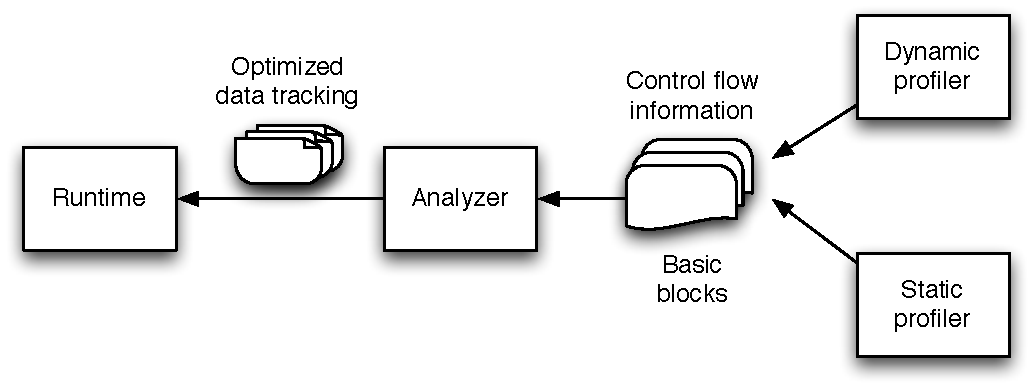
\includegraphics[width=\linewidth]{figs/execution_model.pdf}
    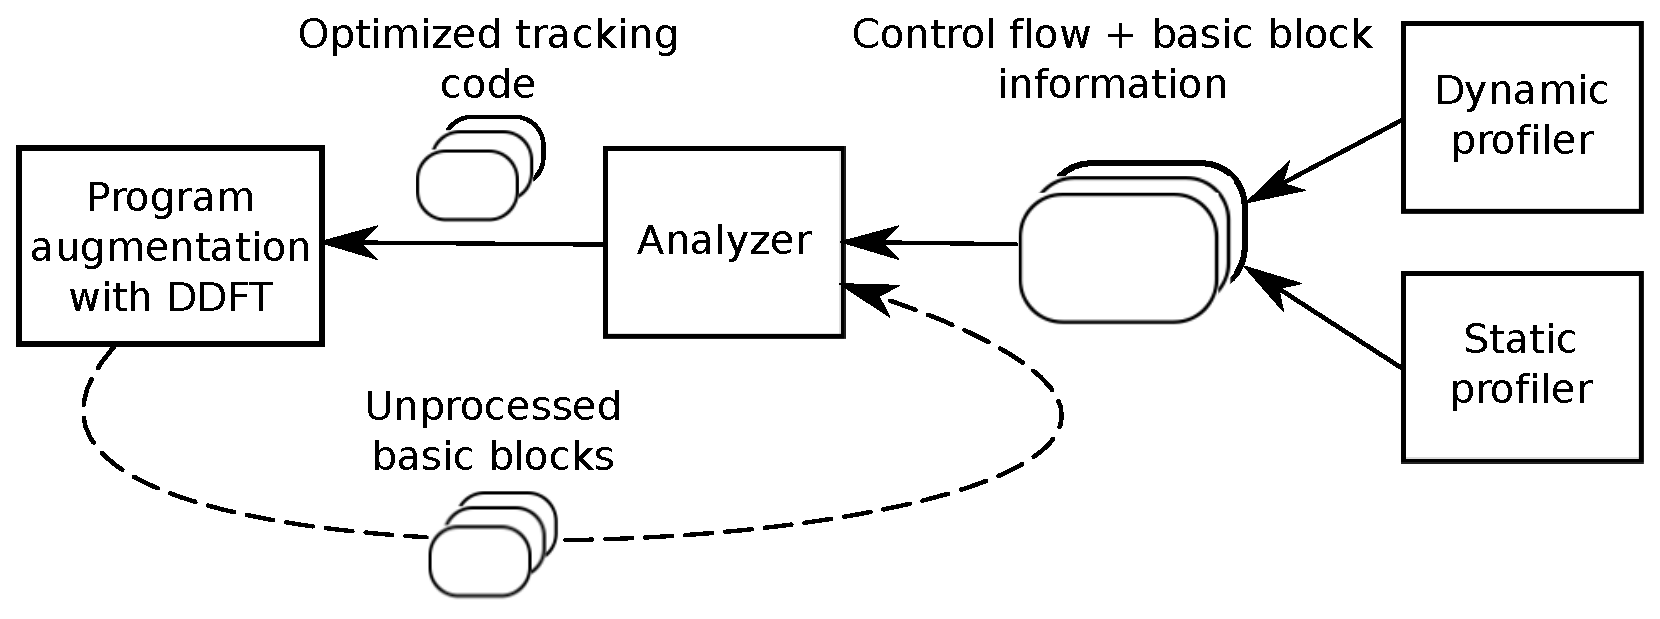
\includegraphics[width=0.6\linewidth]{figs/overview_model.eps}
    \caption{\tfa overview: It extract basic blocks and control flow
    information using a combination of dynamic and static analysis, and then
    statically analyze this information to produce optimized data tracking
    code.
   \label{fig:approach_overview}}
\end{figure}

Figure~\ref{fig:approach_overview} shows a high-level overview of our approach
for optimizing data tracking. We start by dynamically and statically profiling
the target application to extract its basic blocks and control flow
information. A basic block (BBL) of code consists of a sequence of instructions
that has only one entry point and, in our case, a single exit point. This means
that no instruction within a BBL is the target of a jump or branch instruction,
and the block is only exited after its last instruction executes. These
properties are desirable for various types of analysis, like the ones performed
by compilers. The control flow information describes how the basic blocks are
linked. The combination of dynamic and static profiling provides us with a
significant part of the CFG, including the part that dominates in terms of
execution time, and would benefit the most from optimization.
%
The analyzer receives the profiler information and extracts data dependencies
from the code, separating program from data tracking logic. It then transforms
the latter to an internal representation, based on the Taint Flow Algebra
(\tfa), which is highly amenable to various optimizations. The optimizations
performed by the analyzer and include classic compiler optimizations like
dead-code elimination and copy propagation as well as DFT specific ones. Our
goal is to remove redundant tracking operations, and reduce the number of
locations where tracking code is inserted. 
%
Finally, the analyzer emits optimized tracking code, which is applied on the
application. Note that the type of tracking code generated depends on the
original tracking implementation to be optimized. Implementation, as it
operates on binary programs the analyzer produces primitive C code, which can
be compiled and inserted into the application using a DBI framework.

\tfa extends \libdft re-using many features such as instruction interpretation
and shadow memory design. More importantly, \libdft plays a role of slow-path
DFT implementation to cover execution paths missed from static analysis phase
ensuring the completeness of our approach.
 
\subsubsection{\sreplica}
